% Template for ICME-2013 paper; to be used with:
%          spconf.sty  - ICASSP/ICIP LaTeX style file, and
%          IEEEbib.bst - IEEE bibliography style file.
% --------------------------------------------------------------------------
\documentclass{article}
\usepackage{spconf,amsmath,epsfig}

\usepackage[utf8]{inputenc}

% autoref command
\usepackage[hyphens]{url}
\usepackage[pdftex,urlcolor=black,colorlinks=true,linkcolor=black,citecolor=black]{hyperref}
\def\sectionautorefname{Section}
\def\subsectionautorefname{Subsection}
\def\subfigureautorefname{Subfigure}

\pagestyle{empty}

\begin{document}\sloppy

% for 1st, 2nd, etc. superscripting
\newcommand{\ts}{\textsuperscript}

% Title.
% ------
\title{Tell me why! Ain't nothin' but a mistake?\\ Describing Media Item Differences with Media Fragments URI}
%
% Single address.
% ---------------
\name{Anonymous ICME submission}
\address{}

\maketitle

%
\begin{abstract}
We have developed a~tile-wise histogram-based
media item deduplication and clustering algorithm
with additional high-level semantic matching criteria.
In this paper, we investigate whether the addressing scheme
Media Fragments URI provides a~feasible and practicable way
to describe media item differences
between media items of type photo and/or video.
\end{abstract}
%
\begin{keywords}
Media Fragments URI, Media Fragments, Media Items, Deduplication, Social Networks
\end{keywords}
%
\section{Introduction}
\label{sec:introduction}

The \emph{Backstreet Boys}~(BSB) are a~boy band
formed in~1993 in Orlando,~FL
that has sold over 130~million records worldwide,
making them the best-selling boy band of all time.
In~2013, the band will celebrate their 20\ts{th}~anniversary
with a~new album and a~world tour.
Reason enough for us to make them titular saint of this paper
with their hit song \emph{I~Want It That Way}
from the album \emph{Millennium}.
While the spike of their career was in the late 90s,
even today, people still actively share,%
\footnote{BSB on social networks: \url{http://bit.ly/backstreet-gplus}
and \url{http://bit.ly/backstreet-fb},
both accessed 03/04/2013}
publish, and follow the group on \emph{social networks}.

\subsection{Previous Work}
\label{sec:previous-work}

Social networks are at the heart of our research on event summarization,
specifically deduplicating \emph{exact-} and \emph{near-duplicate}
media items that optionally accompany textual status messages
referred to as \emph{microposts} on multiple social networks. 
In the context of our research, we define a~\emph{media item}
as either a~photo (image) or video
that was \emph{publicly} shared or published
on at least one social network.
\autoref{fig:near-duplicate} shows an example
where two users of the social networks Facebook and Google+
independently of each other share a~\emph{near-duplicate} media item
in form of the music video \emph{Everybody}
performed by the \emph{Backstreet Boys}.
In order to detect and cluster such occurrences
of \emph{exact-} and \emph{near-duplicate}
media items being shared independently across social networks,
we have implemented a~tile-wise histogram-based algorithm
with additional high-level semantic matching criteria
that in previous work was shown to work effectively for several events.


\begin{figure}[b!]
  \centering
  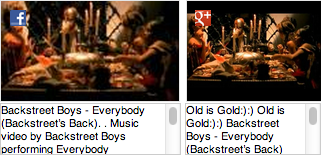
\includegraphics[width=0.5\linewidth]{./backstreetboys.png}
  \caption{\emph{Near-duplicate} music video \emph{Everybody}
    by the \emph{Backstreet Boys} shared
    independently on Facebook and Google+}
  \label{fig:near-duplicate}
\end{figure}

\subsection{Motivation and Research Question}
\label{sec:motivation-and-research-question}

During previous experiments on clustering event-related media items,
we noticed that human raters wanted to know \emph{why}%
\footnote{Tell me why! Ain't nothin' but a mistake?}
certain media items were clustered as \emph{exact-} or \emph{near-duplicates}.
In consequence, in this paper, we investigate in how far
Media Fragments URI~\cite{troncy2012mediafragments}
provides a~feasible and practicable way
to tell raters why media items were clustered.
As we deal with media items of type photo and/or video,
we make simultaneous use of two types of media fragment dimensions,
the temporal dimension and the spatial dimension.

\subsection{Paper Structure}
\label{sec:paper-structure}

The remainder of this paper is structured as follows.


% References should be produced using the bibtex program from suitable
% BiBTeX files (here: strings, refs, manuals). The IEEEbib.bst bibliography
% style file from IEEE produces unsorted bibliography list.
% -------------------------------------------------------------------------
\bibliographystyle{IEEEbib}
\bibliography{icme2013template}

\end{document}
